\documentclass[11pt]{article}
\usepackage{graphicx}
\title{Four-Week Consolidated Strategy Report \\ (As of 2026-04-17)}
\author{Ruiwen HE \and Xin Jin}
\date{\today}

\setlength{\parindent}{0pt}
\setlength{\parskip}{0.7em}

\begin{document}
\maketitle

\section{Executive Summary}
This report is written as a standalone document for readers without access to source code or raw logs.

Over the most recent four official weeks, the baseline model delivered strong absolute return but trailed SPY cumulatively because of two weak middle weeks.

\begin{itemize}
\item Four-week model return (baseline): +5.66\%
\item Four-week benchmark return (SPY): +7.22\%
\item Four-week excess return: -1.56\%
\item Live-to-date return (2026-03-18 to 2026-04-17, baseline): +5.28\%
\item Live-to-date excess return: +1.61\%
\end{itemize}

\section{Strategy Logic, Theory, and Uniqueness}
The strategy is a short-horizon cross-sectional momentum model on a date-consistent S\&P 500 universe.

Each week, it builds the eligible universe for that date, computes momentum scores, selects top-ranked stocks, and holds until the next rebalance.

The model combines cross-sectional momentum persistence, EWMA recency weighting, risk budgeting via volatility targeting, and benchmark-relative evaluation.

\begin{equation}
r_{i,t}=\frac{C_{i,t}}{C_{i,t-1}}-1,
\quad
Score_{i,t}=\sum_{k=0}^{K-1}w_k r_{i,t-k},
\quad
w_k=(1-\lambda)\lambda^k.
\end{equation}

\begin{itemize}
\item Signal at weekly close; execution at next trading session.
\item Current baseline: long-only top 15 names.
\item Week 2 change: fixed 8\% single-name stop-loss activated from 2026-03-30.
\item Week 4 change: added improved diversified variant (about 30 longs).
\end{itemize}

Survivorship bias is controlled by enforcing date-consistent historical membership intervals. At each signal date, only securities that were active index constituents on that date are eligible.

This avoids the common error of backfilling with end-date constituents and keeps historical results academically defensible and operationally realistic.

The strategy is unique because it combines a transparent EWMA alpha engine, strict date-aware universe control, live-governed risk-rule rollout, and side-by-side robustness testing.

\section{Four-Week Performance and Return Curve}
\begin{center}
\small
\begin{tabular}{|l|c|r|r|r|r|}
\hline
Week & Dates & Model & SPY & Excess & PnL \\
\hline
Week 1 & 03/23-03/27 & +5.7748\% & -3.6440\% & +9.4188\% & +\$2.00M \\
\hline
Week 2* & 03/30-04/03 & -2.9339\% & +2.4558\% & -5.3898\% & -\$0.82M \\
\hline
Week 3 & 04/06-04/10 & -2.0280\% & +3.6031\% & -5.6310\% & -\$1.07M \\
\hline
Week 4 & 04/13-04/17 & +5.0433\% & +4.8316\% & +0.2117\% & +\$1.77M \\
\hline
\end{tabular}
\end{center}

\noindent *2026-04-03 was a market holiday (Good Friday), so Week 2 has 4 trading days.

\begin{figure}[h]
\centering
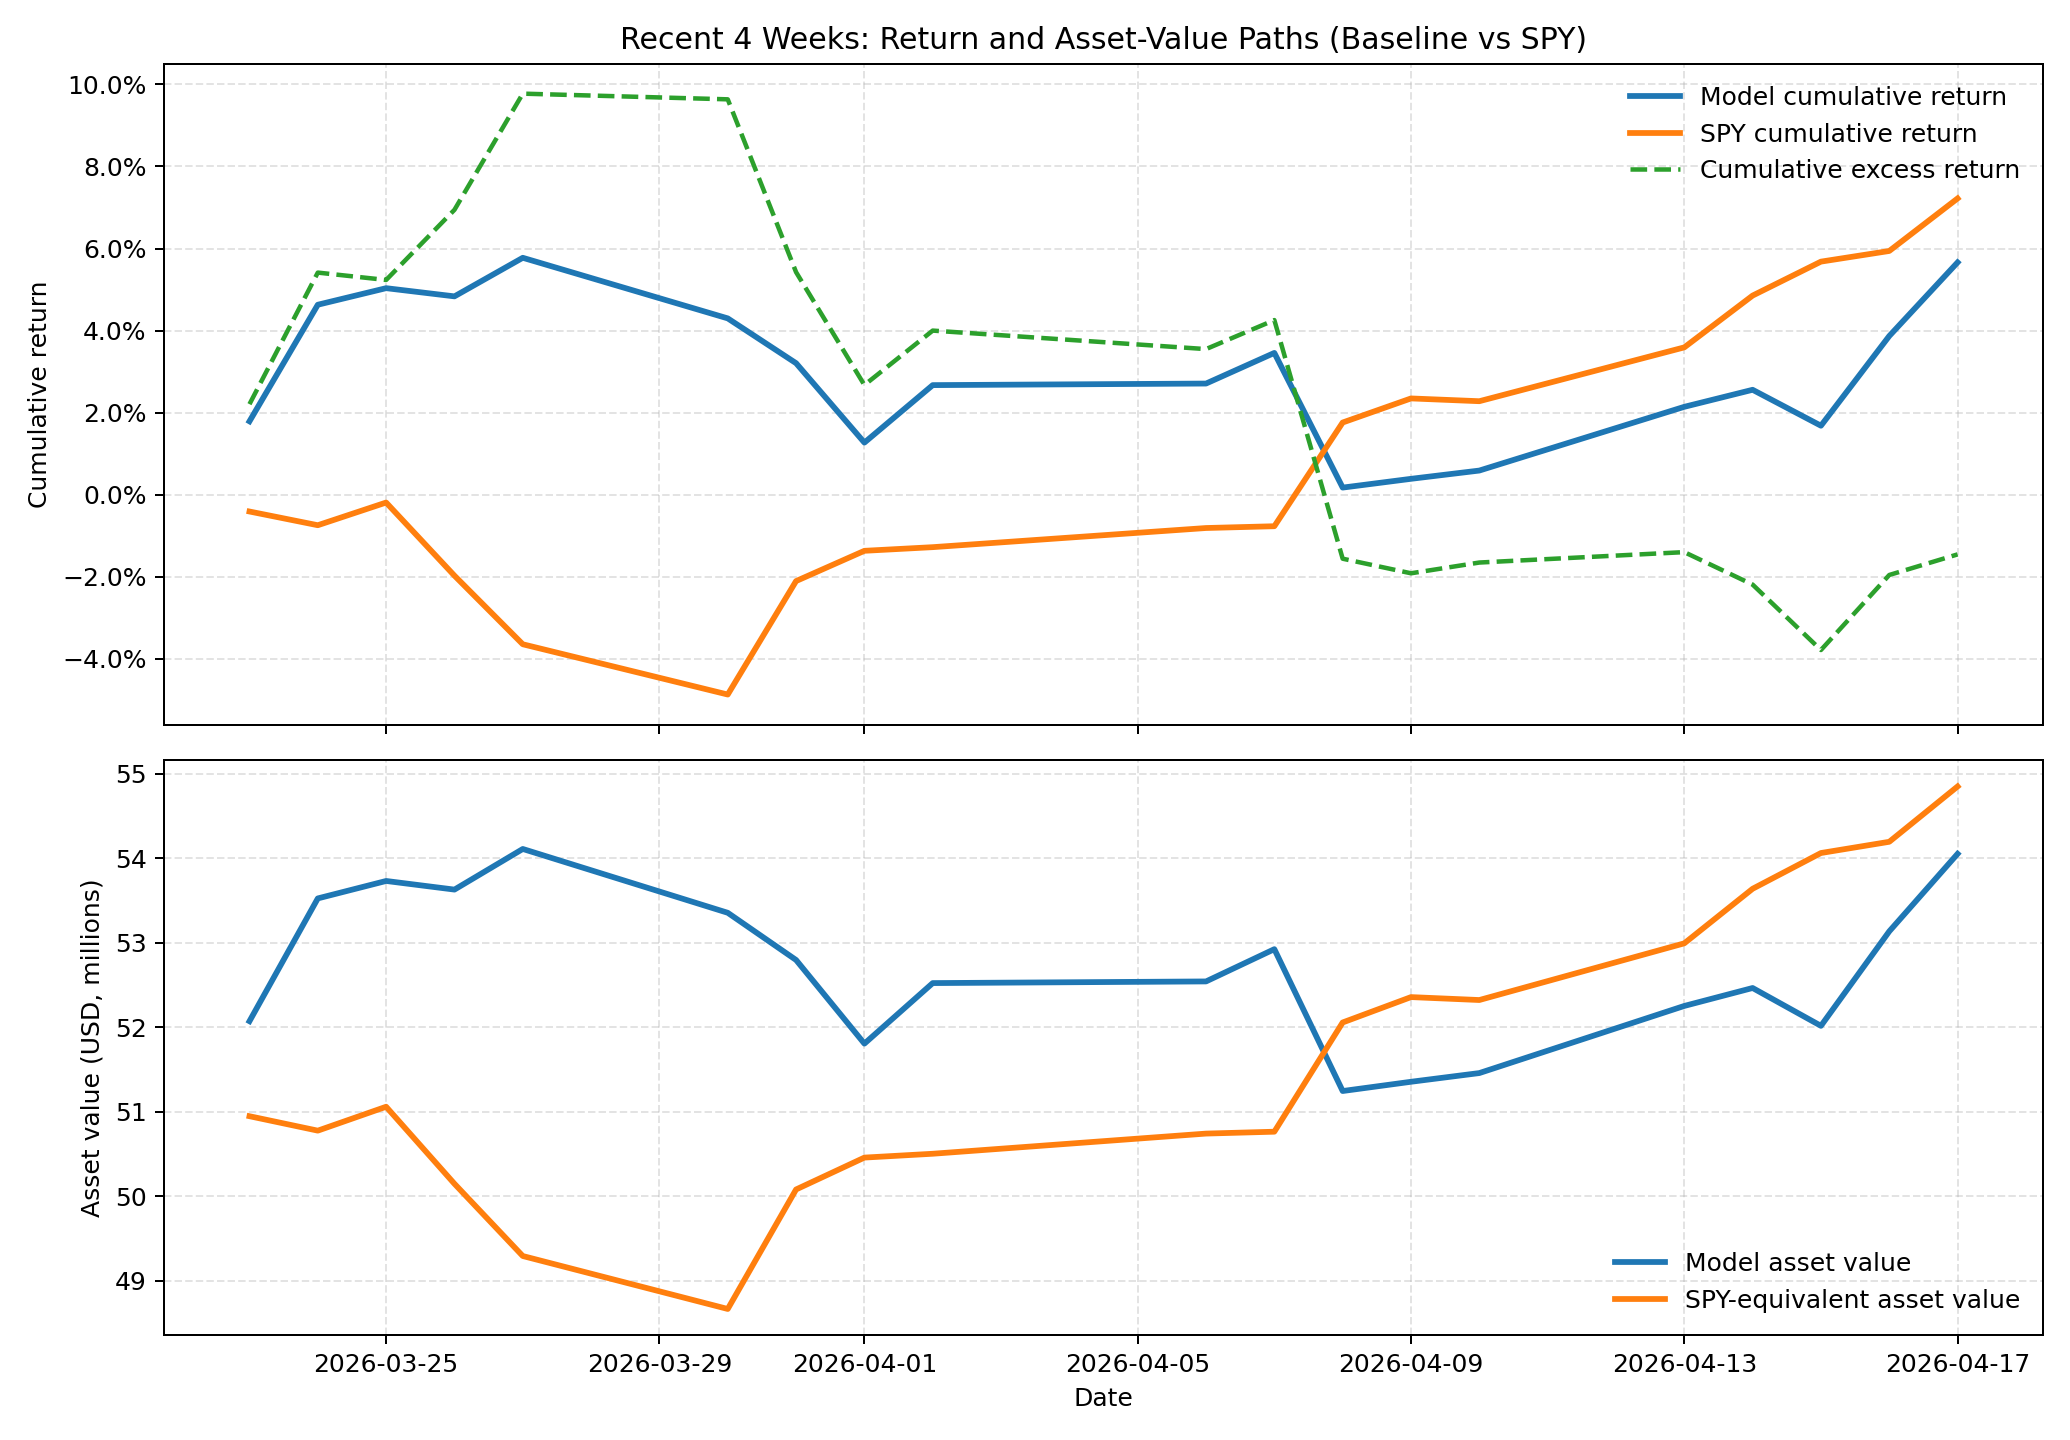
\includegraphics[width=0.95\linewidth]{four_week_multidim_performance_2026-04-17.png}
\caption{Recent 4 Weeks: Multi-Dimensional Performance (Cumulative Return and Asset Value)}
\end{figure}

Top panel: cumulative return paths for baseline, SPY, and cumulative excess return.

Bottom panel: asset-value trajectories for baseline and an SPY-equivalent portfolio with the same initial capital.

In Week 4, the diversified variant returned +4.3812\%, versus baseline at +5.0433\%.

It improved breadth but underperformed in this specific market regime.

\section{Major Up/Down Days and News Attribution}
\textbf{2026-03-31 / 2026-04-01:} Broad risk-on rebound as de-escalation hopes rose; energy lagged as oil eased, which hurt the strategy's then energy-heavy profile.

\textbf{2026-04-08:} Ceasefire-related repricing intensified; benchmark rallied while energy-linked names remained under pressure, producing the worst relative day.

\textbf{2026-04-16:} Semiconductor/AI leadership strengthened (e.g., AMD, LITE, COHR in headlines), aligning closely with baseline holdings and producing strong alpha.

\textbf{2026-04-17:} Strait of Hormuz reopening headlines and sharp oil declines drove broad risk-on behavior and index highs; the model participated with positive excess.

\section{Overall Evaluation, Relative Risk, Forecast, and Next Steps}
Evaluation window for cumulative performance: 2026-03-18 to 2026-04-17.

\begin{itemize}
\item Cumulative model return: +5.28\%
\item Cumulative benchmark return: +3.67\%
\item Cumulative excess return: +1.61\%
\item Sharpe ratio (daily, annualized): 2.68
\item Sortino ratio (daily, annualized): 2.31
\end{itemize}

Interpretation: return and relative alpha are currently positive, with strong short-sample risk-adjusted readings. Statistical confidence remains limited by short history and an event-heavy regime.

Using recent 4-week baseline daily distribution as a proxy:
\begin{itemize}
\item Mean daily return: 0.3009\%
\item Daily volatility: 1.4964\%
\item Implied weekly mean: 1.50\%
\item Implied weekly volatility: 3.35\%
\item Approximate 95\% weekly return interval: [-5.05\%, +8.06\%]
\end{itemize}

Base-case outlook is modestly positive if de-escalation and growth/tech leadership continue; downside risk remains material under abrupt macro regime reversals.

Next improvement priorities:
\begin{enumerate}
\item Add adaptive sector-balance constraints to reduce concentration under regime flips.
\item Introduce tactical hedging triggers for macro stress sessions.
\item Upgrade stop-loss from fixed threshold to volatility-aware trailing control.
\item Blend baseline and diversified variants with a regime-sensitive ensemble weight.
\item Add event-risk calendar filters around geopolitical and macro catalysts.
\item Extend sample length before making stronger statistical claims.
\end{enumerate}

In summary, the strategy's uniqueness lies in combining an intuitive EWMA momentum core with strict implementation discipline. After a volatile four-week path, live-to-date baseline remains positive on both absolute and excess return metrics, while robustness under regime transitions is the primary next objective.

\end{document}
